%\newpage

\subsection{Making Pycket an Independent Racket Implementation}
\label{subsec:pycket}

Pycket is first designed in 2014 as a high-performance JIT compiler
for Racket, generated using the RPython meta-tracing framework
\cite{bolz14-racket}. The language interpreter is based on the CEK
abstract machine and has the state $\langle e, \rho, \kappa \rangle$ ($e$ : control
(program AST), $\rho$ : environment, $\kappa$ : continuation)
\cite{felleisen87}. \figref{fig:cek} shows the transition rules and
how the CEK-loop is implemented in Pycket. The interpreter loop
continuously reduces the CEK triple until an empty continuation is
reached, which triggers a \emph{Done} exception that returns the
results.

\begin{figure}[h!]
  \small
\begin{align*}
e &::= x \mid \lambda x.\, e \mid e \; e\\
\kappa &::= [] \mid \mathsf{arg}(e,\rho){::}\kappa \mid \mathsf{fun}(v,\rho){::}\kappa
\end{align*}
\begin{align*}
\langle x, \rho, \kappa \rangle & \longmapsto
    \langle \rho(x), \rho, \kappa \rangle \\
\langle (e_1 \; e_2), \rho, \kappa \rangle & \longmapsto
    \langle e_1, \rho, \mathsf{arg}(e_2, \rho){::}\kappa \rangle \\
\langle v, \rho, \mathsf{arg}(e,\rho'){::}\kappa \rangle & \longmapsto
    \langle e, \rho', \mathsf{fun}(v,\rho){::}\kappa \rangle \\
\langle v, \rho, \mathsf{fun}(\lambda x. \, e, \rho'){::}\kappa \rangle & \longmapsto
    \langle e, \rho'[x\mapsto v], \kappa \rangle
\end{align*}
\begin{lstlisting}[mathescape]
                                    try:
                                      while True:
                                        ast, env, cont = ast.interpret(env, cont)
                                    except Done, e:
                                      return e.values
\end{lstlisting}
\caption{The CEK Machine transitions and the loop in Pycket. Figure taken from \cite{pycket15}.}
\label{fig:cek}
\end{figure}

In its original design, Pycket relies on the Racket executable to read
and expand a given module into a fully-expanded program
\cite{samth:11}. As shown in \figref{fig:old-pycket}, Pycket runs the
Racket's expander on a given module to fully expand the program, and
then generates AST for it and evaluates it within the interpreter
loop \cite{pycket15}.

\begin{figure}[h!]
  \centering
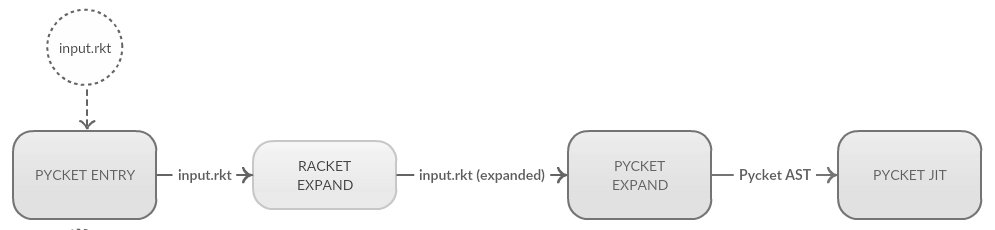
\includegraphics[scale=0.3]{img/old-pycket-grayscale}
\caption{Pycket used to run Racket's expander to fully expand a given module before running it.}
\label{fig:old-pycket}
\end{figure}

Exploiting the increased portability in Racket, here we turn the
Pycket from being a rudimentary compiler to an actual implementation
of Racket, independent of the Racket executable.

First step is building the \emph{linklets} layer by implementing the
\emph{compile-linklet} and \emph{instantiate-linklet} functions in
RPython on the interpreter, thereby allowing Pycket to process and
evaluate linklets. The \emph{compile-linklet} will produce linklet
objects from given linklet s-expressions, creating variables for the
imported and exported variables, processing the body as described in
\secref{subsec:linklet-semantics}. And the \emph{instantiate-linklet}
will carry out the steps for running a linklet, effectively
implementing the $\longrightarrow_{\beta p}$ reduction in the \figref{fig:reduction}
which will be transitively applied by the interpreter loop.

[implementation details?]

After implementing the \emph{compile-linklet} and
\emph{instantiate-linklet}, the next step is to load the bootstrapping
linklets into the run-time as described in
\secref{subsec:racket-portable}. For simplicity, we're only concerned
with loading the \emph{expander} linklet, as it's the most essential
one for bootstrapping (also it's the biggest one). Loading the other
linklets are essentially the same process (modulo the run-time support
they need).

As we described earlier, we run the expander offline on itself using
Racket, which generates a single independent linklet (i.e. no
imports), serialized as an s-expression. Then Pycket runs the
\emph{compile-linklet} function on this s-expression at the very
beginning of its run-time to produce the expander as a runnable
linklet object that exports the aforementioned functionalities such as
read, expand, eval etc into the run-time. At this point, given a
Racket module, Pycket is able to dynamically expand it into a fully
expanded program and run it using the existing CEK interpreter loop.

Ability to run Racket's own expander allows Pycket to run a wide
variety of Racket programs, including the programs in languages built
on top of Racket core, such as \emph{racket/base}, since the expander
also provides the implementation of the macro-system. These programs,
including the bootstrapping linklets themselves often require
additional run-time support such as \emph{correlated} objects (which
are syntax objects without the lexical-content information),
Racket-level exception handling and primitive functions. For example,
in order to have a REPL on Pycket before having Racket's expander in
the run-time, it had to be implemented in RPython. Having the expander
in the run-time allows Pycket to read, expand and run the Racket
program that implements Racket's own REPL without having any
additional RPython implementation. At the same time, the Racket's REPL
implementation requires Racket-level exception handling in the
run-time. The existing Pycket implementation has a rudimentary
exception handling mechanism via transforming the Racket-level
exceptions (which are implemented by Racket structs) into the RPython
exceptions. However, Racket's REPL for example uses the error handling
at the Racket-level, which requires the run-time to support for
installing Racket-level handlers via continuation-marks and
dynamically pass the Racket-level exceptions to the appropriate
handlers.

Moreover, the Racket itself (including the bootstrapping linklets)
generally relies on a large number ($\sim$1500) of primitives, aroud 900
of which we already have in the existing Pycket implementation. An
additional $\sim$200 primitives need to be implemented, along with the
addition of the run-time liblaray \texttt{\#\%linklet} that will
contain 32 linklet related functions including the
\emph{compile-linklet}, \emph{instantiate-linklet} and
\emph{instance-variable-value}.
